\subsection{Co-Simulations and SIL / HIL}

Co-simulations are used to model and analyze complex systems with multiple
interacting components, each of which may have different properties and
behaviors. They involve combining simulation models from different domains, such
as control, power, and thermal management, to create a unified model that
accurately represents the behavior of the overall system.
% outline their use for datacenters with regards to energy systems

One of the main advantages of co-simulations over regular simulations is their
ability to capture the interactions between different components of the system.
Regular simulations often make simplifying assumptions that can lead to
inaccurate results. Co-simulations, on the other hand, can account for the
interactions between components and provide a more accurate representation of
the system's behavior. This makes co-simulations particularly useful for
designing and optimizing complex systems like datacenters. The virtual
environment can save time and resources, reduce the risk of failure, and lead to
more efficient and sustainable datacenters. Furthermore, co-simulations can help
identify potential problems and bottlenecks in the system, allowing to address
them before they become major issues.

\subsection{Mosaik}
%The use of Mosaik brings several benefits compared to traditional simulation
%methods. It offers a more flexible and scalable simulation environment, enabling
%the integration of multiple components and the simulation of large-scale
%systems. Furthermore, it offers a more accurate representation of the energy
%system, incorporating real-world data and parameters, which can be used to
%validate the performance of the Ecovisor.
\subsection{Ecovisor}

\begin{figure}
    \centering
    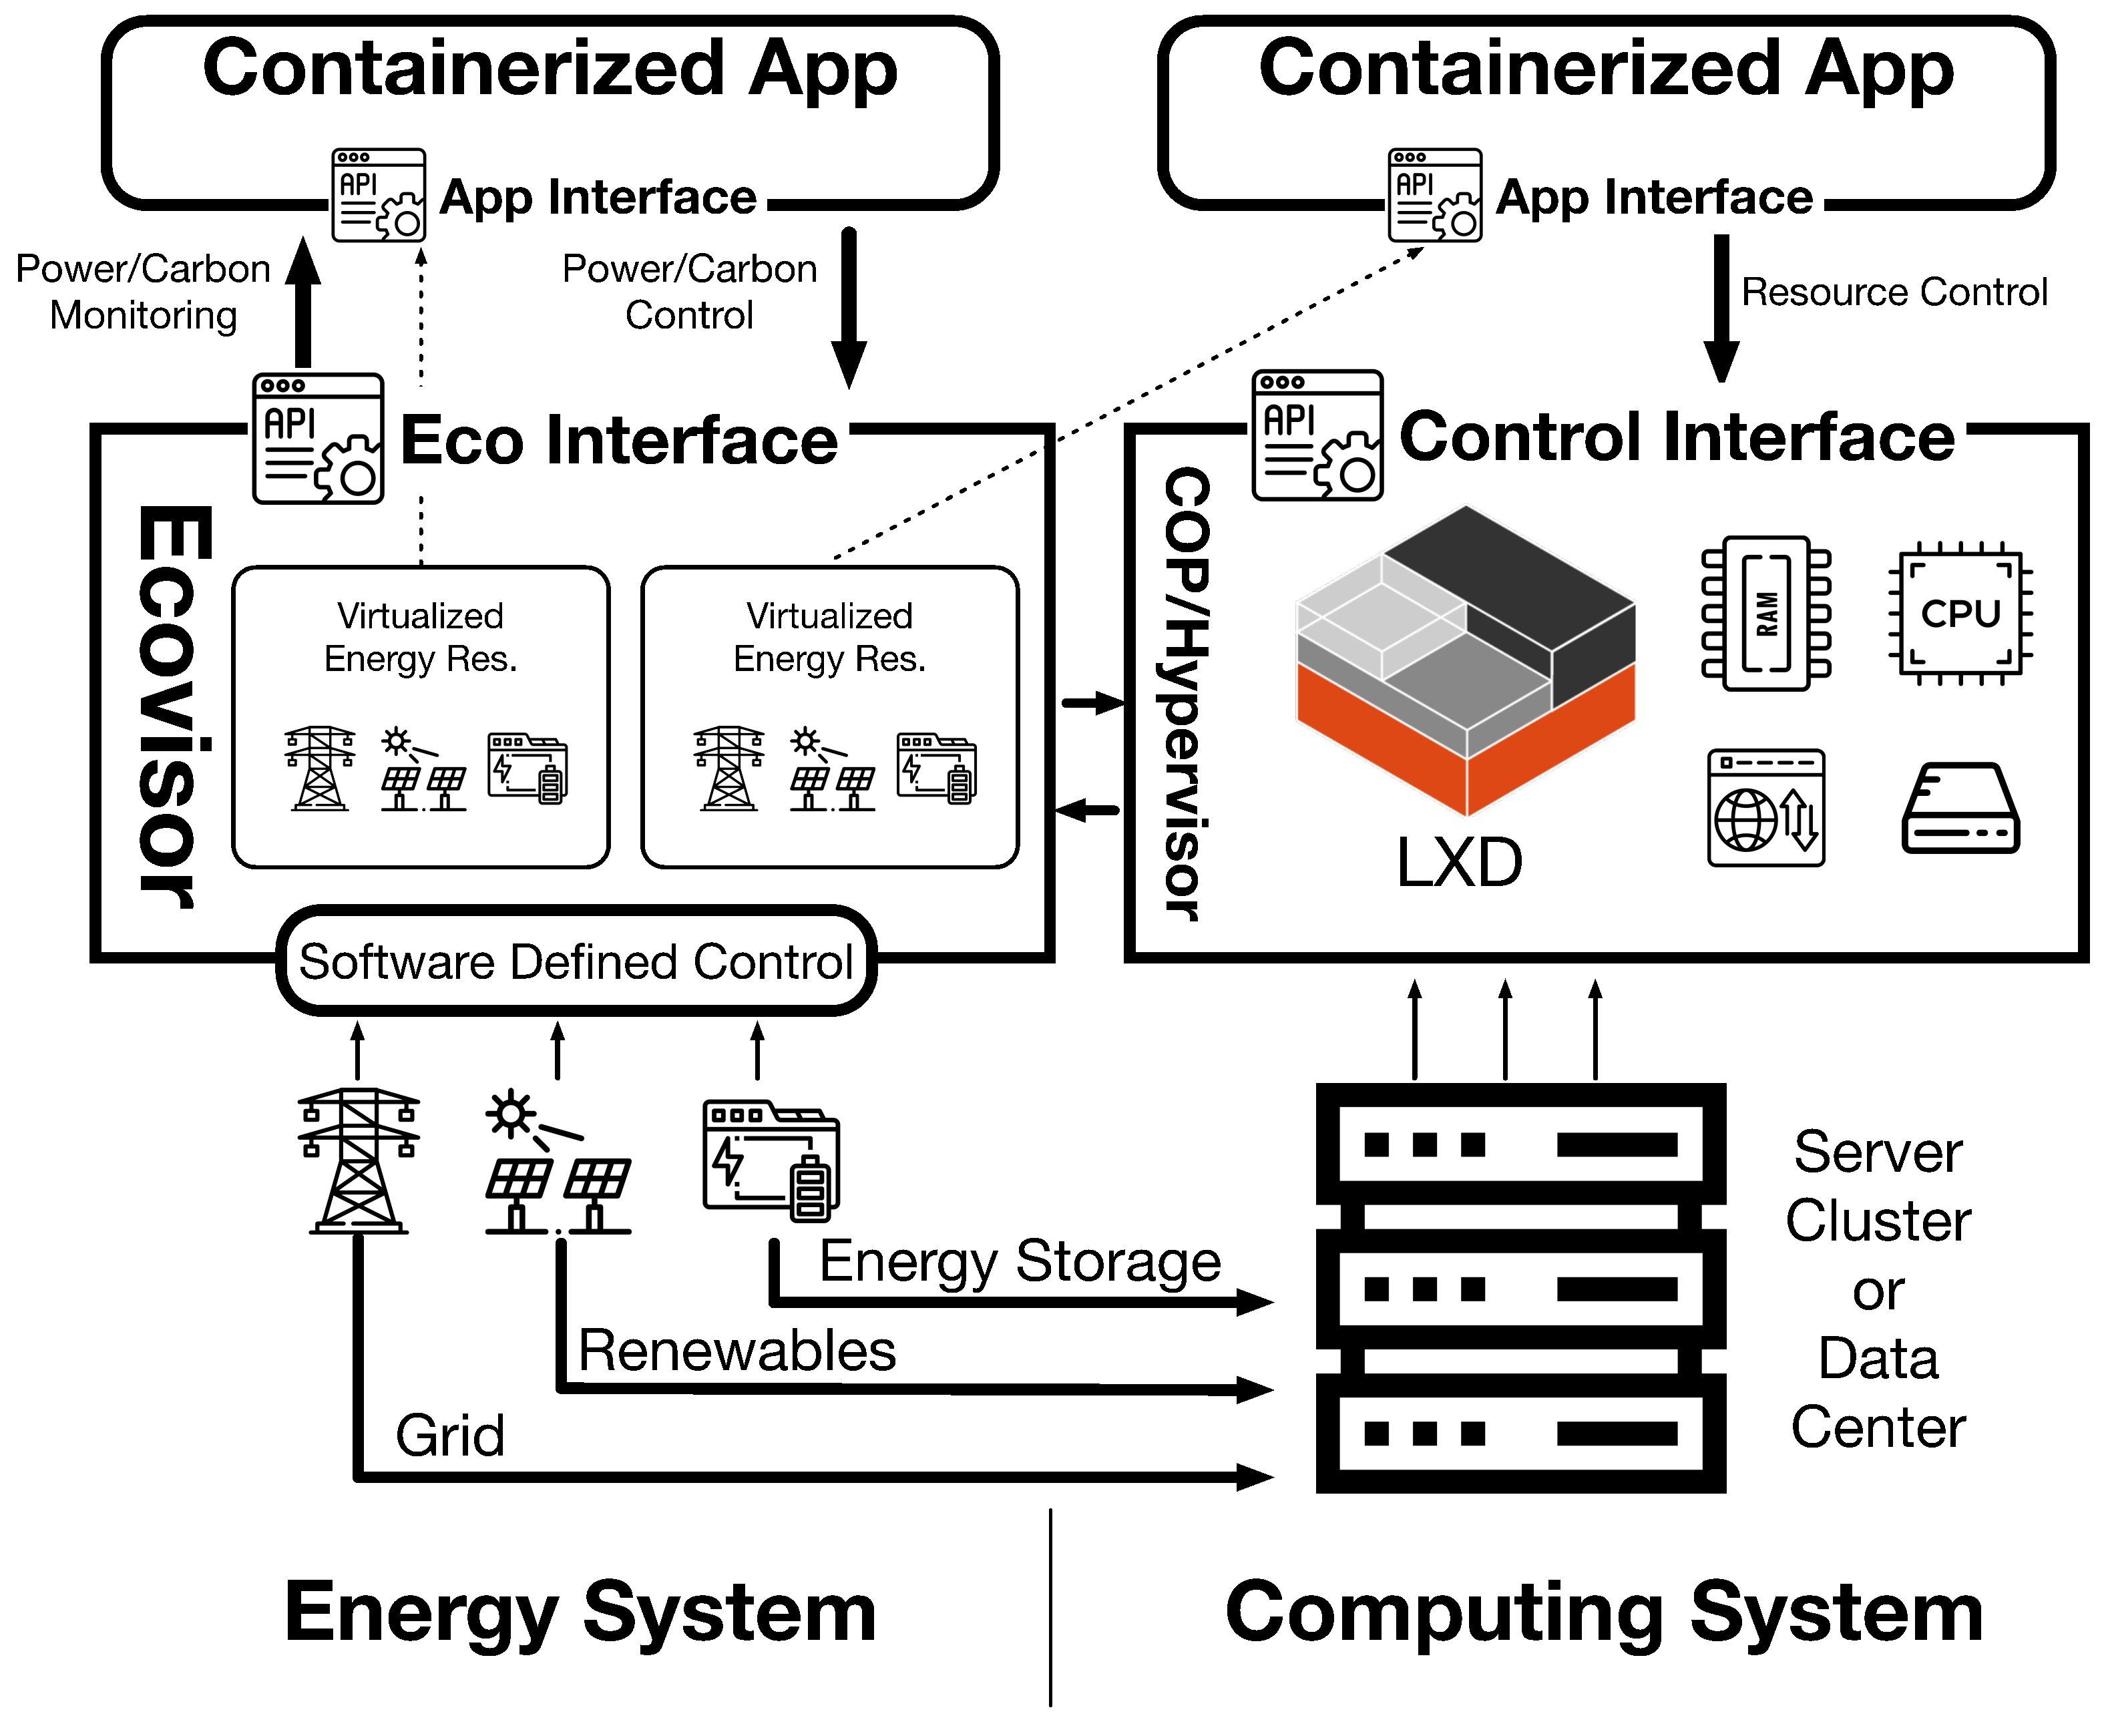
\includegraphics[width=\linewidth]{figures/ecovisor_design}
    \caption{Ecovisor Design (Souza et al.) \cite{souza2023}}
    \label{fig:ecovisor_design}
\end{figure}
